\documentclass{book}
	\usepackage{wrapfig}
	\usepackage{fullpage}
	\usepackage[T1]{fontenc}
	\usepackage[utf8]{inputenc}
	\usepackage{amsfonts}
	\usepackage{amsmath, amssymb, amsthm}
	\usepackage[polish]{babel}
	\usepackage{latexsym}
	\usepackage[pdftex]{graphicx}
	\usepackage{ifthen}
	\usepackage{ulem} % podkreślenia
	\usepackage{icomma} % brak automatycznych spacji po przecinku -- przydatne przy polskich ułamkach
	\usepackage[pdfborder={0 0 0},pdftitle={Automaty a logika}]{hyperref} % linki w spisie treści
	\usepackage{eso-pic}
	\usepackage{graphicx}
	\usepackage{polski}

	\NeedsTeXFormat{LaTeX2e}


\title{Automaty a logika}
\renewcommand{\leq}{\leqslant}
\renewcommand{\geq}{\geqslant}

%dla automatów:
\newcommand{\Aa}{\mathcal A}
\newcommand{\Bb}{\mathcal B}
\newcommand{\Cc}{\mathcal C}

%zbior
\newcommand{\set}[1]{\{#1\}}

\newcommand{\liczby}[1]{\mathbb{#1}} %taką czcionką piszę zbiór liczb
\newcommand{\liczbyR}{\mathbb{R}}
\newcommand{\liczbyQ}{\mathbb{Q}}
\newcommand{\liczbyN}{\mathbb{N}}
%\newcommand{\akapit}{$\: \: \; \;$}
\newcommand{\kwadrat}{ $\quad \square$ \newline \vspace{4ex}}
\newcommand{\kropka}{\cdotp}
\newcommand{\abs}[1]{\left|#1\right|} 
\newcommand{\kwadratd}{ \begin{flushright}
$\quad \square$
\end{flushright} \vspace{4ex}}


\newcounter{zad}[section]
\newcounter{rozw}

%% theorem environments for amsthm

%\theoremstyle{plain}
\newtheorem{twierdzenie}{Twierdzenie}
\newtheorem{lemat}[twierdzenie]{Lemat}
\newtheorem{wniosek}[twierdzenie]{Wniosek}
\newtheorem{fakt}[twierdzenie]{Fakt}
\newtheorem{definicja}{Definicja}


\newcommand{\koniec}{ $\Box$}
 \newenvironment{dowod}[1][!*!,!]%
 {\noindent{\bf Dowód%
     \ifthenelse{\equal{#1}{!*!,!}}{}{%
       \normalfont\ (#1)}\\}}%
 {\koniec\medskip}

\usepackage{comment}


\newif\ifzrozwiazaniami

%\newenvironment{zadanieenv}{{\noindent \bf \thechapter.\thezad.} \stepcounter{zad}}{\bigskip }
\newtheorem{zadanieenv}{Zadanie}[chapter]
%{{\noindent \bf \thechapter.\thezad.} \stepcounter{zad}}{\bigskip }

\newcommand{\zadanie}[4]
{
	
	\ifzrozwiazaniami  % na koncu skryptu
  	 	\ifthenelse{\equal{#2}{}}
		{ % jesli nie ma rozwiazania to nic
		}
		{ % jesli jest rozwiazanie to je wypisujemy
			\label{rozw#2}
			\noindent{\bf Zadanie~\ref{#2}. }#1
	
			\medskip
			\noindent{\bf Rozwiązanie. } (Zapisał #3.)

			\medskip
			\noindent #4
			\vfill \pagebreak
		}
	\else  % po rozdziale
		\begin{zadanieenv}\label{#2}
			#1
			\ifthenelse{\equal{#2}{}}
			{  % brak rozwiazania
			}
			{  % jest rozwiazanie
				\smallskip
				\noindent{\it Rozwiązanie na stronie \pageref{rozw#2}.}
			}	
		\end{zadanieenv}
	\fi



}
\specialcomment{rozwiazanie}{\begin{proof}}{\end{proof}}
\excludecomment{rozwiazanie}

\newenvironment{rbody}%
{\noindent{\bf Rozwiązanie:}\vskip 0.05cm}%
{\medskip}

\newenvironment{przyklad}{\noindent{\bf Przykład. }}{~$\square$}
\newenvironment{uwaga}{{\bf Uwaga. }}{}

\newcommand{\cwiczenia}{
\ifzrozwiazaniami
\else
\setcounter{zad}{1} \pagebreak
{\noindent \large \bf Zadania} \bigskip
\fi}



\newcommand{\spisali}[1]{\vspace{-1,2cm} Spisali: #1
\vspace{1cm}}
\newcommand{\spisal}[1]{\vspace{-1,2cm} Spisał: #1
\vspace{1cm}}
\newcommand{\spisala}[1]{\vspace{-1,2cm} Spisała: #1
\vspace{1cm}}

\newcommand{\HRule}{\rule{\linewidth}{0.2mm}}

\newcommand\BackgroundPic{
\put(0,0){\includegraphics[width=\paperwidth,height=\paperheight]{background.png}}%
}

\newcommand\okladka{

\newpage
\thispagestyle{empty}
\phantom{v}
\newpage
}


\begin{document}
\pagestyle{plain}
\thispagestyle{empty}

\begin{center}

\textsf{\Large Wydział Matematyki, Informatyki i~Mechaniki UW}
\vskip 2.5cm

\HRule \vskip 0.5cm
{\Huge \bfseries \textsf{Algebraiczna Teoria Języków}}
\linebreak \vskip 0.2cm 
{\large \bfseries \textsf{skrypt z wykładu i ćwiczeń}}
\vskip 0.1cm
\HRule \vskip 2.5cm

{\large \textsf{semestr zimowy 2010/2011}}
\end{center}
\vfill
\newpage
\thispagestyle{empty}
\begin{center}
\begin{tabular}[width=\textwidth]{ l l}
 {Przedmiot prowadzili} & Mikołaj Bojańczyk\\ & Tomasz Idziaszek\\&  Paweł Parys
    \\ \\
{Teksty spisali}
 & Paweł Pasteczka\\
 & Krzysztof Gogolewski \\
 & Marcin Kotowski \\
 & Michał Kotowski \\
 & Michał Bendowski \\
 & Katarzyna Krasnowska \\
 & Michał Żak \\
 & Dariusz Leniowski \\
 & Adam Witkowski \\
 & Michal Jatrzebski \\
 & Bartosz Lewinski \\
 & Piotr Leszczyński \\
 & Maria Donten-Bury \\
 & Tomasz Kulczyński \\
 & Tomasz Weksej \\
 \\ \\
 {Rozdziały zaakceptowane} & 1, 2, 3
\end{tabular}
\end{center}
\newpage



\tableofcontents

\chapter{Języki ścieżkowe i logika temporalna}
\spisali{Tomek Kulczyński i Tomek Weksej}

\section{Języki pełnościeżkowe}

\begin{definicja}
	Język pełnościeżkowy to booleowska kombinacja języków postaci
	$$\mathrm{E}^{\textrm{liść}}L.$$
\end{definicja}

Sformułujemy teraz twierdzenie analogiczne do \ref{tw:sciezkowe}, charakteryzujące języki pełnościeżkowe poprzez ich algebrę syntaktyczną. Zauważmy najpierw, że twierdzenie w wersji dla języków ścieżkowych to rzeczywiście zbyt mało --- problematyczna jest tu równość $(ii)$: gdy za $g$ podstawimy pusty las otrzymamy:

$$v(0+h) = v0 + vh,$$

czyli

$$vh = v0 + vh.$$

Od razu widać, że ta równość niekoniecznie musi być spełniona, gdyż zbiór \textit{ścieżek liściowych} (pełnych ścieżek korzeń -- liść) prawej strony równości może być istotnie większy od zbioru pełnych ścieżek lewej strony.

Musimy więc nieco wzbogacić to twierdzenie, co uczynimy poniżej.

\begin{twierdzenie}
	Niech $L \subseteq H_A$ będzie regularnym językiem lasów. Niech $(H_L, V_L)$ będzie jego algebrą syntaktyczną. Następujące warunki są równoważne:
	
	\begin{enumerate}[(a)]
		\item $L$ jest językiem pełnościeżkowym
		\item $(H_L, V_L)$ spełnia:
		\begin{enumerate}[(i)]
			\item $h + g = g + h$ dla $h,g \in H_L$\label{(i)}
			\item $v(g+h) = vg + vh$ dla $v \in V_L$, $g,h \in H_L$, o ile $g,h$ są obrazami niepustych lasów\label{(ii)}
			\item $h + h = h$, dla $h \in H_L$.\label{(iii)}
		\end{enumerate}
	\end{enumerate}
\end{twierdzenie}

Poczyńmy kilka obserwacji:

\begin{fakt}
	Tak jak w przypadku języków ścieżkowych, równanie (\ref{(iii)}) jest konsekwencją równań (\ref{(i)}) oraz (\ref{(ii)}).
\end{fakt}

\begin{fakt}\label{fakt:homomorfizm}
	W odróżnieniu od języków ścieżkowych, rozstrzygnięcie czy dany język jest językiem pełnościeżkowym wymaga badania nie tylko algebry syntaktycznej, ale też homomorfizmu syntaktycznego.
\end{fakt}

Zatrzymajmy się na chwilę nad faktem \ref{fakt:homomorfizm}. Zauważmy, że modyfikacja twierdzenia \ref{tw:sciezkowe} polegała na dodaniu do równości (\ref{(ii)}) założenia ,,o ile $g,h$ są obrazami niepustych lasów''. Rzeczywiście opisuje to homomorfizm, a nie algebrę. Aby zilustrować ten fakt, przyjrzyjmy się następującemu przykładowi.

\begin{przyklad}
	Przedstawimy dwa języki spośród których tylko jeden jest językiem pełnościeżkowym. Oba za to mają taką samą algebrę syntaktyczną.
	
	\begin{itemize}
		\item $L = \textrm{,,istnieje liść $a$''},$ $A = \{a,b\}$,
		\item $L' = \textrm{,,po usunięciu $c$ istnieje liść $a$''},$ $A = \{a,b,c\}$.
	\end{itemize}
	
	Przez ,,usunięcie $c$'' rozumiemy następującą operację:
	
	\begin{center}
		\begin{minipage}[t]{.25\linewidth}
			\vspace{0pt}
			\centering
			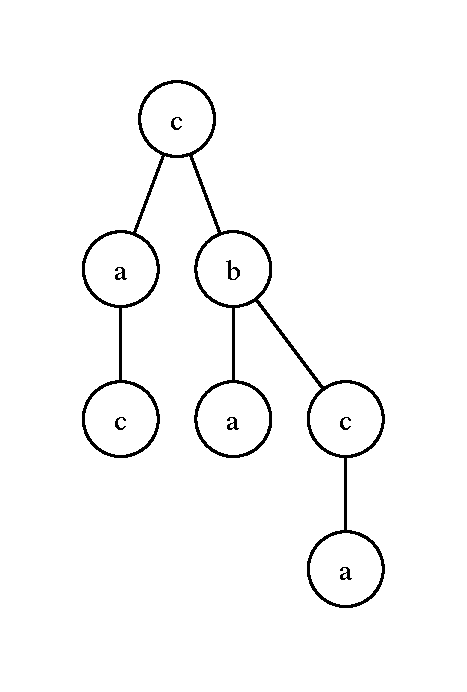
\includegraphics[scale=0.6]{rysunki/w12-usuniecie_c_1.pdf}
		\end{minipage}
		\begin{minipage}[t]{.25\linewidth}
			\centering 
			\vspace{40pt}
			\begin{displaymath}
				\xymatrix{ 
					\ar@{~>}[rr]^{\textrm{usunięcie $c$}} &&
				}
			\end{displaymath}
		\end{minipage}
		\begin{minipage}[t]{.25\linewidth}
			\vspace{0pt}
			\centering
			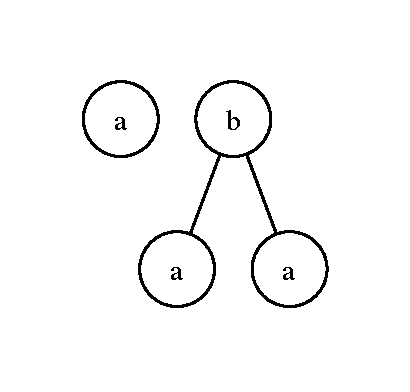
\includegraphics[scale=0.6]{rysunki/w12-usuniecie_c_2.pdf}
		\end{minipage}
	\end{center}
	
	Oczywiście $L$ jest językiem pełnościeżkowym. Oba te języki mają taką samą algebrę syntaktyczną --- danemu $t' \in L'$ przypisany jest ten sam element algebry co odpowiadającemu mu $t \in L$ (tzn. osiągniętym przez usunięcie $c$).
	
	$L'$ nie jest za to językiem pełnościeżkowym. Rozpatrzmy przedstawione poniżej lasy $t_1$ (po lewej) oraz $t_2$. Odpowiadający im zbiór ścieżek liściowych jest taki sam (a więc jest im przyporządkowany ten sam element algebry syntaktycznej), ale $t_1 'in L'$, a $t_2 \notin L'$.
	
	\begin{center}
		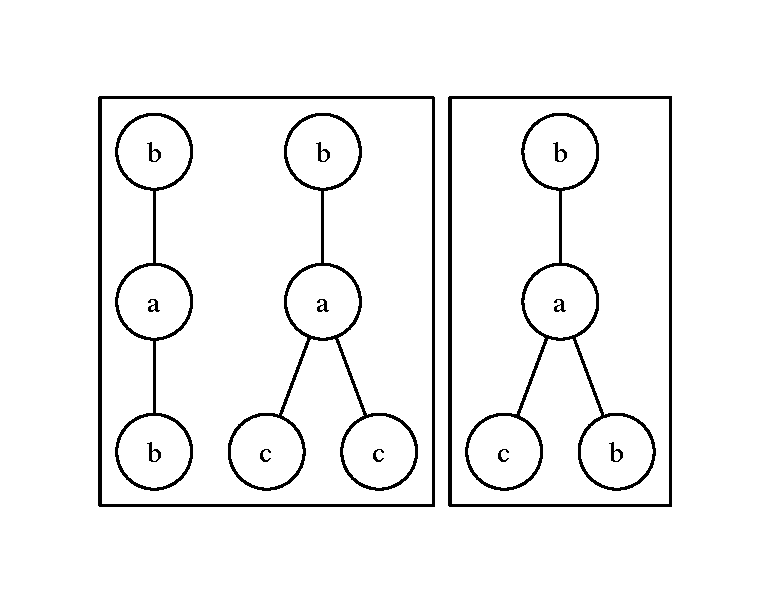
\includegraphics[scale=0.6]{rysunki/w12-l_prim.pdf}
	\end{center}
	
\end{przyklad}

\end{document}
      
